\documentclass{article}
\usepackage{geometry}
\geometry{a4paper, margin=1in}
\usepackage{array}
\usepackage{tabularx}
\usepackage{booktabs}
\usepackage{graphicx}
\graphicspath{ {../assets/} }

\title{Development Plan\\\progname}

\author{\authname}

\date{}

%% Comments

\usepackage{color}

\newif\ifcomments\commentstrue %displays comments
%\newif\ifcomments\commentsfalse %so that comments do not display

\ifcomments
\newcommand{\authornote}[3]{\textcolor{#1}{[#3 ---#2]}}
\newcommand{\todo}[1]{\textcolor{red}{[TODO: #1]}}
\else
\newcommand{\authornote}[3]{}
\newcommand{\todo}[1]{}
\fi

\newcommand{\wss}[1]{\authornote{blue}{SS}{#1}} 
\newcommand{\plt}[1]{\authornote{magenta}{TPLT}{#1}} %For explanation of the template
\newcommand{\an}[1]{\authornote{cyan}{Author}{#1}}

%% Common Parts

\newcommand{\progname}{ProgName} % PUT YOUR PROGRAM NAME HERE
\newcommand{\authname}{Team \#, Team Name
\\ Student 1 name
\\ Student 2 name
\\ Student 3 name
\\ Student 4 name} % AUTHOR NAMES                  

\usepackage{hyperref}
    \hypersetup{colorlinks=true, linkcolor=blue, citecolor=blue, filecolor=blue,
                urlcolor=blue, unicode=false}
    \urlstyle{same}
                                

The purpose of reflection questions is to give you a chance to assess your own
learning and that of your group as a whole, and to find ways to improve in the
future. Reflection is an important part of the learning process.  Reflection is
also an essential component of a successful software development process.  

Reflections are most interesting and useful when they're honest, even if the
stories they tell are imperfect. You will be marked based on your depth of
thought and analysis, and not based on the content of the reflections
themselves. Thus, for full marks we encourage you to answer openly and honestly
and to avoid simply writing ``what you think the evaluator wants to hear.''

Please answer the following questions.  Some questions can be answered on the
team level, but where appropriate, each team member should write their own
response:


\begin{document}

\maketitle

\begin{table}[hp]
\caption{Revision History} \label{TblRevisionHistory}
\begin{tabularx}{\textwidth}{llX}
\toprule
\textbf{Date} & \textbf{Developer (s)} & \textbf{Change}\\
\midrule
Sep 16, 2024 & Ayman & Fixed Strcuture of DEV PLAN \\
Sep 16, 2024 & Ayman & Updated Sections Iteration one\\
Sep 18, 2024 & Nathan & Dev plan nathan\\
Sep 18, 2024 & Kelly & Add section 1, 4\\
Sep 19, 2024 & Patrick & Q2, Q10 \\
Sep 19, 2024 & Nathan & Escape special characters\\
Sep 20, 2024 & Reza & Section 10 (Expected Technology)\\
Sep 20, 2024 & Patrick & TeamCharter Update\\
\bottomrule
\end{tabularx}
\end{table}

The Development Plan document outline our group approach to the development of the CXR project. The document includes, and not limited to, our team operation and technical standard to drive the project forward, and on-time. These standards includes: standardized tool, communication plan, individuals responsibility, development standards, and Proof of Concept planning. Team members are committed to carry out the development plan listed below, with the supervision and approval of Dr.Mehdi Moradi.

\newpage{}

\section{Confidential Information}

As we are not using real patient data, all the data we are using is publicly available and open-source. However, the data we are using is not to be used for commercial purposes. Furthermore, in the future if we decide to use real patient data, we will need to ensure that the data is anonymized and that we have the necessary permissions to use it. We will also need to comply with all relevant privacy laws and regulations to protect the confidentiality of the data.
\section{IP to Protect}

This section outlines the terms of use and intellectual property rights related to the technologies used in this project, including Python, NumPy, PyTorch, CheXpert, and TypeScript. By using these technologies, all contributors acknowledge and agree to abide by the associated licenses and intellectual property terms.\\
\textbf{Licences}
\begin{itemize}
    \item \href{https://docs.python.org/3/license.html#psf-license}{Python}
    \item \href{https://numpy.org/terms/#:~:text=These%20Terms%20of%20Use%20constitute,mobile%20website%20or%20mobile%20application}{NumPy}
    \item \href{https://discuss.pytorch.org/tos}{PyTorch}
    \item \href{https://www.stanford.edu/site/terms/}{CheXpert}
    \item \href{https://www.typescriptlang.org/License.html}{TypeScript}
\end{itemize}
\textbf{Acknowledgement of Terms}\\
By contributing to or using this project, I acknowledge that I have read, understood, and agree to abide by the intellectual property rights. I understand the limitations and permissions granted under these licenses and commit to proper attribution and compliance with the terms of use for each technology.

\vspace{1em} % Adds space between paragraphs

\noindent
Contributor Signature: \underline{\texttt{LZ KD AA NL RJ}} \hspace{4cm} Date: \underline{Sept 6 2024}

\section{Copyright License}

Our Team is adopting an MIT License, which is a permissive open-source license. This license  allows users to freely use, copy, modify, merge, publish, distribute, sub-license, and even sell copies of the software, provided that the original copyright notice and the license text are included with all copies or substantial portions of the software. The license can be found in our GitHub repository at the link below.

\begin{itemize}
    \item Link: \url{https://github.com/RezaJodeiri/CXR-Capstone/blob/main/LICENSE}
\end{itemize}

\section{Team Meeting Plan}

Our team plans to meet twice a week on Discord (virtual meetings) to discuss upcoming deliverables and development progress on AI models. 
Our team plans to meet with the supervisor at least once a month via Teams. In the meetings our team plans to update the supervisor about our current progress, what challenges we are facing, what are the next steps and what advice does the instructor has. 


\section{Team Communication Plan}

Neuralyzers plans to hold in person and virtual meetings as a method of communication between the team. 

\subsection{Discord}
Discord will be used as the team's main method of communication as its great at message logging, file sharing, creating threads for issues, real time communication and creating channels to separate information. Discord will be used by team members to update, and send key information or documentation links such as GitHub links, YouTube links, and code blocks to help keep the team up to date as well as ensure note taking is kept at a high standard. 
\subsection{GitHub}
GitHub is a great resource that Neuralyzers will be utilizing to create branches and track code whilst ensuring clean merging of code between members. On GitHub, issue requests can be created for the team to be notified and add input, to fix following issues as well as update the project as a whole. This will be the key center point where all the documentation and code will be saved. 

\section{Team Member Roles}

\begin{itemize}
\item Nathan Luong
    \begin{itemize}
        \item Scrum Master
        \item Developer
        \item Machine Learning Expert: Will do research on how to effectively read the X-Ray Image and create models that can be used to read race, age, and details of the patient. 
    \end{itemize}
    \item Ayman
    \begin{itemize}
        \item Developer
        \item Note Taker
        \item Computer Vision Expert: Will do research on how using Pytorch or Cuda could be utlized to ensure best performance of Application. 
    \end{itemize}
\item Patrick Zhou
    \begin{itemize}
        \item Developer
        \item Reviewer
        \item Python Expert: Will be in charge of Documentation of Python code Labeling each Function as well as, keeping the programming style consistent. Will be able to transform our pseudo-code into Python code. 
    \end{itemize}
        
\item Kelly Deng
    \begin{itemize}
        \item Developer
        \item Meeting Chair
        \item Machine Learning Expert: Will do research on how to effectively read the X-Ray Image and create models that can be used to read race, age, and details of the patient. 
    \end{itemize}
\item Reza Jodeiri
    \begin{itemize}
        \item Developer
        \item Leader 
        \item Chest X-ray Expert: Will lead the research and guide the team towards achieving the project’s objectives through their deep understanding of chest X-rays. Their expertise will be instrumental in ensuring that the X-ray images are accurately interpreted, identifying key anomalies and common disease patterns. This knowledge will directly contribute to training the machine learning model by selecting the most relevant features and markers for disease detection, such as abnormalities in lung structure, nodules, or lesions. 
    \end{itemize}
\end{itemize}
  
\section{Workflow Plan}

\begin{itemize}

  \item Usage of Git, GitHub
  \begin{itemize}
    \item The capstone repository (https://github.com/RezaJodeiri/CXR-Capstone) will be actively maintained by all 5 members.
    \item Many Core GitHub features will be used extensively in order to drive our capstone project.
    \begin{itemize}
      \item \textbf{GitHub Issues}: to track Issues, tickets, bugs, and tasks.
      \item \textbf{GitHub Projects}: to track monitor project progress, and important deadline management.
      \item \textbf{GitHub Repository}: to monitor, and track changes, and store source code of the capstone project.
      \item \textbf{GitHub Actions}: to run automation for continuous integration tasks. For example: Unit tests or linting check per pull requests.
      \item \textbf{GitHub Branch Protection}: to protect developers from accidental code push onto main branch.
      \item \textbf{GitHub Approval Rules}: to make sure that changes are approved by all 4 other team members, before being merged into main.
    \end{itemize}
  \end{itemize}

  \item Pull Requests
  \begin{itemize}
    \item All Pull Requests will come with a template. This template can be found under \begin{verbatim}.github/pull_request_template.md \end{verbatim}
    \item On every pull requests, members are required to provide detail descriptions, and checklist, ensuring standardized code-review process.
  \end{itemize}
  
  \item Branching Strategy
  \begin{itemize}
    \item Branching Strategy might differ from case-to-case. However, general development guideline will encourage members to follow a trunk-based development approach.
    \item Each members will be responsible to keep their local repositories up-to-date with the remote repository, then each member will work on the ticket/issue/task, and open a pull request against the main branch.
    \item With this branching strategy, each team members would need to perform rebasing on a regular basics, to avoid big merge conflicts, and potential efficiency lost. 
    \item The branch name should be descriptive of the change that being developed. For example: \texttt{dev\_plan\_MEMBER\_NAME} or \texttt{feature/training-data-labelling}

  \end{itemize}
	
	\item Issues/ Tickets Tracking \& Management
  \begin{itemize}
    \item Issues tracking and management will be conducted via GitHub Issues. We chose this platform instead of Jira or Trello, since GitHub can be a one-stop-shop, and preventing context switching for team members.
    \item Each issue must contain a tag (ie documentation, bug, duplicate, feature-request) to classify the issue type.
    \item Each issue must contain an assignee, and the assignee is responsible to investigate and close the issue.
  \end{itemize}

  \item Usage of Continuous Integration / Continuous Deployment
  \begin{itemize}
    \item As mentioned, GitHub Actions will be used for CI/CD automation.
    \item CI/CD can be utilized for unit testing, linting, security checks, automatic deployment onto cloud environment (AWS, GCP).
    \item CI/CD automation would need to be developed in conjunction with feature development in order to reduce human error, and repetitive work.
  \end{itemize}

\end{itemize}

\section{Project Decomposition and Scheduling}

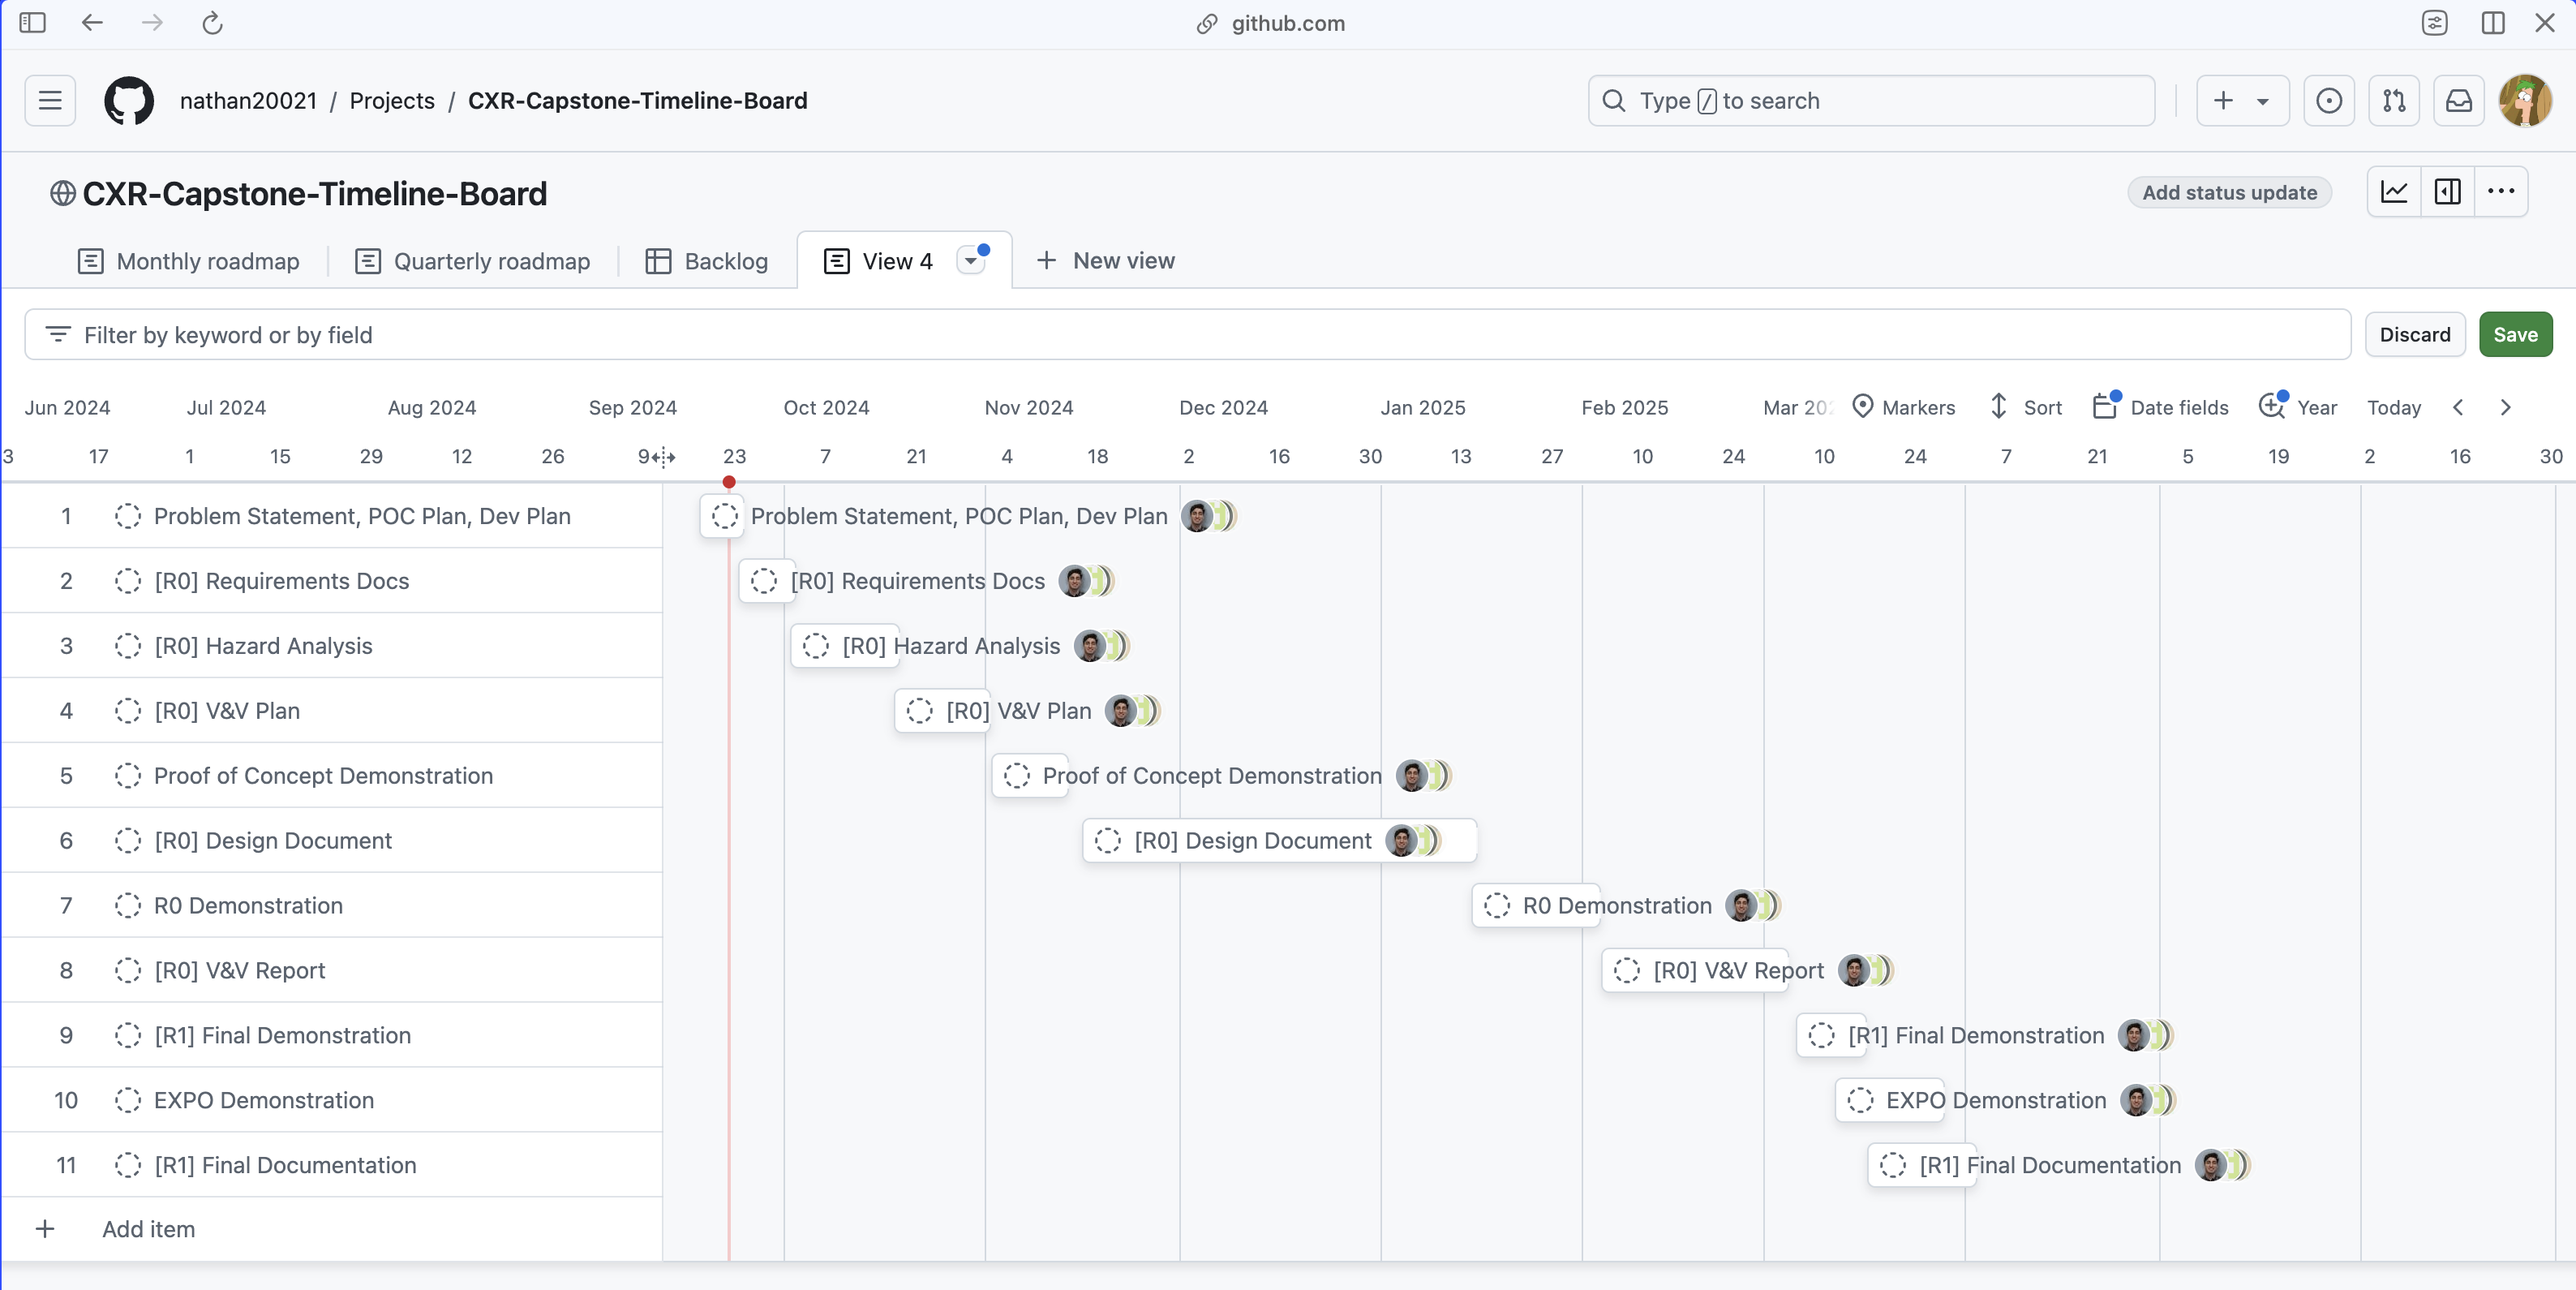
\includegraphics[scale=0.3]{prelim-timeline.png}
\begin{itemize}
    \item How will you be using GitHub projects? 
    \begin{itemize}
        \item We will be using GitHub Project to monitor and manage status of tasks, and TODO items.
        \item Our GitHub Project board has been pre-populated with deadlines from the Course Outline, public link provided below. 
        \item We will create a project board with columns such as To Do, In Progress, and Done. Each task will be represented as an issue on the project board. The project board will be updated regularly to reflect the current status of the project.
    \end{itemize}
    \item GitHub Project Link 
    \begin{itemize}
        \item Project Board View \url{https://github.com/users/nathan20021/projects/3/views/4}
        \item Roadmap View \url{https://github.com/users/nathan20021/projects/3/views/4?layout=roadmap}
    \end{itemize}
\end{itemize}



\section{Proof of Concept Demonstration Plan}
\subsection{Risks}
With many moving parts in the application, our Proof of Concept Demo Plan involves critical components and tasks that carry risks if not implemented correctly. These risks are:

\begin{itemize}
    \item Inability to Confidently Identify Diseases:
    \begin{itemize}
        \item Description: The pre-trained, open-source model (e.g., TorchXRayVision) may not achieve sufficient accuracy (below 80\%) in identifying diseases from chest X-rays.
        \item Concern: Low accuracy could undermine the system's reliability, potentially impacting clinical decision-making and causing delays or misdiagnoses.
        \item Mitigation Strategy: If the model underperforms, we will switch to a more clinically validated model, such as CheXNet, which has higher reported accuracy in chest X-ray classification. We will also run cross-validation tests on a smaller dataset to benchmark models before integration.
    \end{itemize}

    \item Insufficient Access to Test Data for Model Validation:
    \begin{itemize}
        \item Description: Gathering diverse and labeled X-ray data for testing and validation might be challenging.
        \item Concern: Incomplete or insufficient data could skew our understanding of the model’s performance, affecting its generalizability in real-world use cases.
        \item Mitigation Strategy: If test data is limited, we will explore alternative datasets like MIMIC-CXR or NIH Chest X-ray Dataset to validate our results.
    \end{itemize}

    \item High Latency in Image Processing:
    \begin{itemize}
        \item Description: The system may experience delays when processing large chest X-ray images, especially with multiple users accessing the system at the same time.
        \item Concern: High latency could slow down results, which might affect the system’s usability in clinical settings.
        \item Mitigation Strategy: We will resize images where possible, utilize GPU acceleration, and implement parallel processing. Additionally, load balancing and caching mechanisms will be used to reduce any bottlenecks during high traffic periods.
    \end{itemize}

    \item Challenges with Hosting Application in a Cloud Environment:
    \begin{itemize}
        \item Description: Hosting the application in a cloud environment may encounter technical issues like compatibility, networking, or scaling.
        \item Concern: Without cloud hosting, scalability and accessibility of the app may be limited during demonstrations and deployment.
        \item Mitigation Strategy: If cloud hosting proves infeasible, we will deploy the application locally for the demonstration. Testing will be conducted both on cloud environments (e.g., AWS, Google Cloud) and locally to ensure smooth fallback if issues arise.
    \end{itemize}
\end{itemize}

\subsection{Demonstration Plan}
\begin{itemize}
    \item For the Proof of Concept, our team would like to achieve the following high-level goals:
    \begin{itemize}
        \item Clearly define the project's problem statement.
        \item Demonstrate a simple cloud-native web application (Architectural diagram provided below) that is capable of:
        \begin{itemize}
            \item Accepting input as an Chest X-Ray image, returns the disease label associating with it (Lung Lesion, Hernia, Edema, etc.), as well as certain image labels (race, age, etc.).
            \item Handling data transfer securely with Bearer authorization mechanism, allowing only authenticated application can interact with the ML model.
            \item Providing a user-friendly interface to interact with the Machine Learning service.
            \item Providing the ability to swap out the pre-trained model with self-trained ones with ease and minimal downtime.
        \end{itemize}
    \end{itemize}
    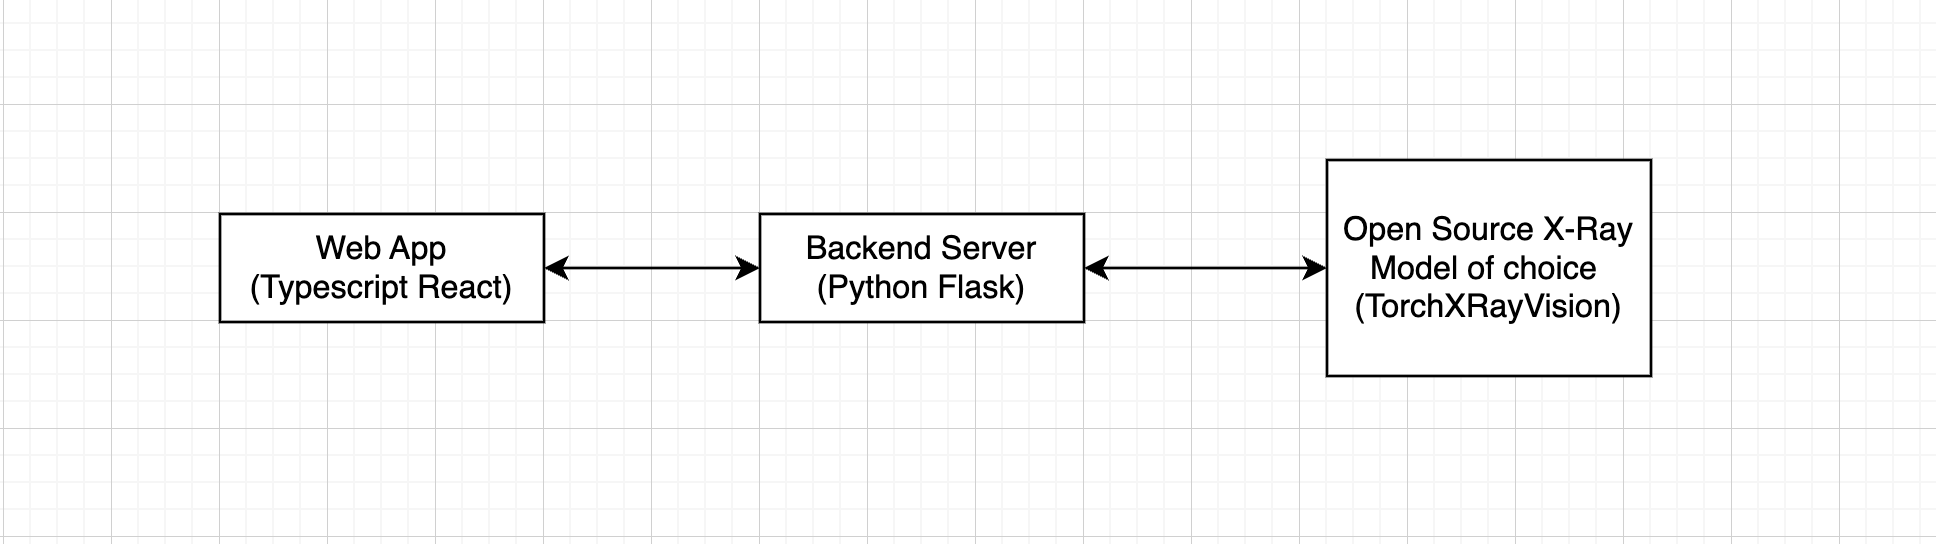
\includegraphics[scale=0.45]{poc-architectural-diagram.png}
    
    \item Possible Technical Deliverables:
    \begin{itemize}
        \item First iteration source code of:
        \begin{itemize}
            \item A web-based front-end application, written in TypeScript, with the ability to upload images and returning a label.
            \item A back-end server (written in Python) that interacts with the front-end application and Machine Learning Server.
            \item A pre-trained, open-source Chest X-ray machine learning model that can be called via some cloud-native protocol (HTTP, or gRPC).
            \item Github Actions files that automates software testing and full-stack deployment on public cloud provider of choice.
        \end{itemize}
    \end{itemize}
\end{itemize}
\newpage
\section{Expected Technology}
\renewcommand{\arraystretch}{1.5} 
\begin{table}[h!]
    \centering
    \begin{tabularx}{\textwidth}{| >{\raggedright\arraybackslash}m{3.5cm} | >{\raggedright\arraybackslash}X |}
        \hline
        \textbf{Component} & \textbf{Technology / Description} \\ \hline
        \textbf{Programming Language} & \begin{itemize}
          \item \textbf{Python}: Chosen for its extensive support for machine learning and medical imaging libraries and models.
          \item \textbf{JavaScript}: For developing the web-based user interface and interactive visualization components that allows users to upload chest X-ray images and view the results of the AI model.
          \item \textbf{Groovy/Bash}: For writing scripts to automate the deployment of the application and setting up CI/CD pipelines.
      \end{itemize} \\ \hline 
        \textbf{Machine Learning Framework} & \textbf{PyTorch}: Selected due to its flexibility, dynamic computation graphs, and support for GPU acceleration, which are essential for training deep learning models on large datasets. \\ \hline
        \textbf{Medical Imaging Libraries} & \begin{itemize}
            \item \textbf{TorchXRayVision}: To leverage pre-trained models and Chest X-ray datasets such as CheXpert and tools specifically designed for medical image analysis, particularly chest X-rays. 
            \item \textbf{scikit-learn}: For additional image pre-processing tasks like resizing and normalization.
        \end{itemize} \\ \hline
        \textbf{Pre-trained Models} & \textbf{ResNet}: Utilized as a backbone architecture for transfer learning to classify chest X-ray images. Pre-trained models will be fine-tuned on the project’s dataset(Imagenome) to yield desired accuracy and performance. \\ \hline
        \textbf{Linter Tool} & \textbf{Pylint}: To ensure code adheres to Python's coding standards and improve code quality through automated static analysis. \\ \hline
        \textbf{Unit Testing Framework} & \textbf{Pytest}: For writing and automating tests to verify the reliability and functionality of machine learning models and components. \\ \hline
        \textbf{Code Coverage Tool} & \textbf{Coverage.py}: Integrated with Pytest to measure the percentage of code covered by unit tests, ensuring robust testing of the codebase. \\ \hline
        
        \textbf{Continuous Integration} & \textbf{GitHub Actions}: Automates testing, linting, and other checks when code is pushed to the repository. \\ \hline
        \textbf{Development Environment} & \begin{itemize}
          \item \textbf{Visual Studio Code}: Chosen for its extensive Python support, ease of use, and integration with GitHub for version control and collaboration.
          \item \textbf{Docker}: To containerize our packages and dependencies, ensuring consistency across different environments and simplifying deployment.
      \end{itemize}\\ \hline
        \textbf{Documentation Tool} & \textbf{LaTeX/Overleaf}: For writing and formatting our capstone documents, reports, and deliverables. \\ \hline
    \end{tabularx}
    \caption{Technology Choices for Capstone Project}
\end{table}

\newpage
\section{Coding Standard}
During the development of the project, we will adhere to the following standards to maintain readable and high-quality code. All Python files (.py) will conform to the PEP 8 style guide. Similarly, TypeScript files (.ts) will follow the Google TypeScript Style Guide. The reformatting tools will be employed to enforce these coding standards automatically. By adhering to these guidelines, we aim to ensure consistency across the codebase, improve readability, and facilitate easier maintenance and collaboration among team members.

\section*{\href{https://github.com/python/cpython}{Python}}

\textbf{Standard:} \href{https://peps.python.org/pep-0008/}{PEP 8 – Style Guide for Python Code} \\
\textbf{Code Formatter:} \href{https://github.com/hhatto/autopep8}{Autopep8} \\
\textbf{Example Function:} \texttt{\href{https://github.com/pytorch/pytorch/blob/main/torch/cpu/__init__.py}{pytorch/torch/cpu/\_\_init\_\_.py}} \\\\
All Python files (\texttt{.py}) in the project will adhere to the PEP 8 style guide to maintain readability and consistency in the codebase.

\subsection*{PEP 8 Key Principles}

\begin{itemize}
    \item \textbf{Indentation:} Use 4 spaces per indentation level.
    \item \textbf{Maximum Line Length:} Limit all lines to a maximum of 79 characters.
    \item \textbf{Blank Lines:} Use blank lines to separate functions and classes, as well as larger blocks of code inside functions.
    \item \textbf{Imports:} Group imports in the following order:
    \begin{enumerate}
        \item Standard library imports,
        \item Related third-party imports,
        \item Local application/library-specific imports.
    \end{enumerate}
    Each group should be separated by a blank line.
    \item \textbf{Spaces:} Avoid extraneous white space in expressions and statements (e.g., immediately before a comma, colon, or semicolon).
    \item \textbf{Naming Conventions:}
    \begin{itemize}
        \item Use \texttt{snake\_case} for function and variable names.
        \item Use \texttt{CapitalizedWords} for class names.
    \end{itemize}
\end{itemize}

\subsection*{Code Formatting with Autopep8}

To enforce these practices, Autopep8 will be used as the automatic code formatter. Autopep8 will automatically adjust formatting issues in Python code to conform to the PEP 8 style guide. This tool will help ensure consistent style and quality throughout the project by reformatting the code according to PEP 8 rules.

\subsection*{Usage}

To use Autopep8 for formatting:\\
\texttt{autopep8 --in-place --aggressive --aggressive <filename>.py}\\\\
This command applies formatting to a specific Python file.

\newpage{}

\section*{\href{https://github.com/microsoft/TypeScript}{TypeScript}}

\textbf{Standard:} \href{https://google.github.io/styleguide/tsguide.html}{Google TypeScript Style Guide} \\
\textbf{Code Formatter:} \href{https://github.com/prettier/prettier}{Prettier} \\
\textbf{Example Function:} \texttt{\href{https://github.com/angular/angular/blob/main/devtools/projects/ng-devtools/src/lib/devtools_spec.ts}{angular/devtools/projects/ng-devtools/src/lib/devtools\_spec.ts}} \\\\
All TypeScript files (\texttt{.ts}) in the project will follow the Google TypeScript Style Guide to maintain a high level of consistency and readability across the codebase.

\subsection*{Key Principles from the Google TypeScript Style Guide}

\begin{itemize}
    \item \textbf{Indentation:} Use 2 spaces per indentation level.
    \item \textbf{Maximum Line Length:} Limit all lines to a maximum of 80 characters.
    \item \textbf{Semicolons:} Always use semicolons to terminate statements.
    \item \textbf{Quotes:} Use single quotes (\texttt{'}), except to avoid escaping.
    \item \textbf{Naming Conventions:}
    \begin{itemize}
        \item Use \texttt{camelCase} for variable, function, and method names.
        \item Use \texttt{PascalCase} for class and interface names.
    \end{itemize}
    \item \textbf{Type Annotations:} Prefer explicit type annotations where possible.
    \item \textbf{Imports:} Organize imports into groups:
    \begin{enumerate}
        \item Standard libraries,
        \item Third-party dependencies,
        \item Local modules.
    \end{enumerate}
    Each group should be separated by a blank line.
    \item \textbf{No Trailing Commas:} Avoid trailing commas in arrays, objects, and function parameters.
\end{itemize}

\subsection*{Code Formatting with Prettier}

To enforce these style guidelines, Prettier will be used as the code formatter. Prettier will automatically format TypeScript code to conform to the Google TypeScript Style Guide rules, ensuring consistent styling across the project.

\subsection*{Usage}
To use Prettier for formatting:  \texttt{prettier --write <filename>.ts}\\\\
This command applies formatting to a specific TypeScript file.

\newpage{}

\section*{Appendix --- Reflection}

\begin{enumerate}
    \item Why is it important to create a development plan prior to starting the
    project?
    \begin{itemize}
        \item It is crucial to create a development plan prior to starting the project as it aims to ensure that the project is completed on time and within budget. The development plan outlines the tasks that need to be completed, the resources that are required, and the timeline for completion. By creating a development plan, the team can identify potential risks and issues early on and develop strategies to mitigate them. The development plan also helps to ensure that all team members are on the same page and working towards the same goals.
    \end{itemize}
    \item In your opinion, what are the advantages and disadvantages of using
    CI/CD? \\ \\
    % \begin{itemize}
        Advantages of using CI/CD include:
        \begin{itemize}
        \item Improved code quality: CI/CD runs automated tests on the code to identify bugs and issues early on, which can help to improve the overall quality of the code.
        \item Faster Development: By using CI/CD we can encourage/create faster development cycles that automate the process of building, testing, and deploying code, which can help to speed up the development process.
        \item Reduced Human Error: By making the deployment process automated, the chance manual errors when deploying is significantly reduced, ensuring reliability and consistency in releases.
        \end{itemize}
    % \end{itemize}
    \item What disagreements did your group have in this deliverable, if any,
    and how did you resolve them?
    \begin{itemize}
        \item Our group did not have any disagreements in this deliverable.
    \end{itemize}
\end{enumerate}

\newpage{}

\section*{Appendix --- Team Charter}

\subsection*{External Goals}
The reason why we chose this project because we aim to accomplish more than just completing a "project". It involves neural networks, meaning we'll need to build our own model at some stage, as freshman which has no knowledge in this field, we have a couple things we are looking to achieve during the development. \\\\
1. Learning about AI \\
This project offers a unique opportunity to dive deep into the world of artificial intelligence, particularly neural networks. Under the mentorship of Dr. Mehdi, an expert in AI, we are looking to absorb as much knowledge as possible as noobies in this field. We aim to learn concepts and build something meaningful from ground up.\\\\
2. Creating Real Impact \\
We aspire to go beyond the typical boundaries of a student project, instead of merely completing an assignment, we want to create a functional product that has the potential to be used by real customers. Meaning that our project can help real-life medical X-Ray analysis. \\\\
3. Developing a High-Standard Product \\
We are fully committed to investing the time and effort necessary to ensure that the final product meets a high standard of quality. Our vision is to create something we can genuinely be proud of, something that stands out. Like an art piece for an artist.
\subsection*{Attendance}

\subsubsection*{Expectations}
As part of our expectations for the project, we plan to meet with Dr. Mehdi on a weekly basis to report our progress and receive feedback. We will also maintain an issue board that tracks our tasks, helping us stay organized and focused. Each week, our team will meet to review the current tasks, provide updates, create new tasks, and address any blockers or decide if certain tasks need to be adjusted or canceled. While the exact number of work hours is not yet determined, our goal is to maximize productivity and ensure steady progress throughout the project.


\subsubsection*{Acceptable Excuse}
Some acceptable reasons for missing team meetings or deadlines include:
\begin{itemize}
    \item \textbf{Sick leave}: If a team member is unwell, they can take time off to recover.
    \item \textbf{Family emergencies}: In urgent family situations, such as medical emergencies or significant personal matters.
    \item \textbf{Pre-approved personal time}: If a team member has informed the team in advance about personal commitments, like travel or important appointments.
    \item \textbf{Technical difficulties}: When technical issues, such as hardware failure or internet outages, prevent participation.
    \item \textbf{Academic obligations}: If academic work, such as exams or major assignments, requires immediate attention and has been communicated in advance.
\end{itemize}

\subsubsection*{In Case of Emergency}

In case of emergency, we will reassign the task from the member who has been affect to other members. Or adjust the workload expected for the affected member respectfully.\\

\subsection*{Accountability and Teamwork}

\subsubsection*{Quality} 

We expect that during the meeting, each team member will have their own task to complete or will actively contribute to solving the group problem. To ensure code quality and maintain standards, we will conduct code reviews. The overall quality standard for the project will be determined by the professor's satisfaction with the final product, meaning we will have met the expectations if the professor is pleased with the outcome.

\subsubsection*{Attitude}

Our team values a positive and collaborative attitude from all members. We expect:
\begin{itemize}
    \item \textbf{Respect for ideas}: Every member's input is valued, and differing opinions are encouraged to foster innovation.
    \item \textbf{Cooperation and teamwork}: Members should be supportive and willing to help each other to achieve common goals.
    \item \textbf{Constructive feedback}: Feedback should be given and received in a respectful and constructive manner.
    \item \textbf{Positive attitude}: A can-do mindset and a willingness to adapt to challenges are key to maintaining team morale.
\end{itemize}
We may (if someone reports violation of above values) adopt a formal code of conduct and establish a conflict resolution plan to ensure a harmonious and productive working environment. In the current stage we expect everyone to behave nicely and following these rules.

\subsubsection*{Stay on Track}

To ensure our team stays on track, we will implement the following methods:\\\\
\textbf{Progress Reports}: We will regularly report project metrics during meetings to assess our progress and identify any challenges.\\
\textbf{Target Metrics}: Each team member will have specific tasks to finish or deadline, each member is responsible for their assigned task.\\\\
To ensure that all members contribute as expected, we will hold periodic reviews to discuss individual contributions and overall team performance. \\\\
\textbf{Recognition and Rewards}: Members who consistently meet or exceed their targets will be recognized in team meetings and mentioned in each checkpoints.\\\\
\textbf{Management of Below-Expectations Performance}: If a member's performance falls below expectations, we will address the issue openly and collaboratively find solutions. Possible consequences may include:
\begin{itemize}
    \item Increased check-ins to provide support.
    \item A requirement to present a progress update at the next team meeting.
    \item A meeting with the TA or instructor if necessary.
\end{itemize}

\subsubsection*{Incentives and Consequences}

We expect to measure performance based on the quality of work produced and the effort invested, rather than setting specific target metrics for attendance, commits, or similar criteria.

\subsubsection*{Team Building}

We build team spirit through a mix of teamwork sessions and external activities, including:
\begin{itemize}
    \item \textbf{Collaboration}: Regular sessions focused on solving challenges together.
    \item \textbf{Social activities}: Group outings or informal gatherings to strengthen bonds.
    \item \textbf{Recognition}: Celebrating achievements to maintain a positive atmosphere.
\end{itemize}

\subsubsection*{Decision Making} 

The group consists of five members, so a majority vote will almost always be possible. We will use this as our standard practice for making important decisions. If a decision is deemed less critical or pertains to an individual's specific tasks, that person can make the decision independently.

\end{document}